%%%%%%%%%%%%%%%%%%%%%%%%%%%%%%%%%%%%%%%%%
% Programming/Coding Assignment
% LaTeX Template
%
% This template has been downloaded from:
% http://www.latextemplates.com
%
% Original author:
% Ted Pavlic (http://www.tedpavlic.com)
%
% Note:
% The \lipsum[#] commands throughout this template generate dummy text
% to fill the template out. These commands should all be removed when 
% writing assignment content.
%
% This template uses a Perl script as an example snippet of code, most other
% languages are also usable. Configure them in the "CODE INCLUSION 
% CONFIGURATION" section.
%
%%%%%%%%%%%%%%%%%%%%%%%%%%%%%%%%%%%%%%%%%

%----------------------------------------------------------------------------------------
%	PACKAGES AND OTHER DOCUMENT CONFIGURATIONS
%----------------------------------------------------------------------------------------

\documentclass{article}

\usepackage{fancyhdr} % Required for custom headers
\usepackage{lastpage} % Required to determine the last page for the footer
\usepackage{extramarks} % Required for headers and footers
\usepackage[usenames,dvipsnames]{color} % Required for custom colors
\usepackage{graphicx} % Required to insert images
\usepackage{subcaption}
\usepackage{listings} % Required for insertion of code
\usepackage{courier} % Required for the courier font
\usepackage{lipsum} % Used for inserting dummy 'Lorem ipsum' text into the template
\usepackage{enumerate}
\usepackage{amssymb}
\usepackage{amsmath}
\usepackage{array}
\usepackage{forloop}
\usepackage{alphalph}
\renewcommand*{\thesubfigure}{%
\alphalph{\value{subfigure}}%
}%
% !TeX spellcheck = en_GB

% Margins
\topmargin=-0.45in
\evensidemargin=0in
\oddsidemargin=0in
\textwidth=6.5in
\textheight=9.0in
\headsep=0.25in

\linespread{1.1} % Line spacing

% Set up the header and footer
\pagestyle{fancy}
\lhead{\hmwkAuthorName} % Top left header
\chead{\hmwkClass\ (\hmwkClassTime): \hmwkTitle} % Top center head
%\rhead{\firstxmark} % Top right header
\lfoot{\lastxmark} % Bottom left footer
\cfoot{} % Bottom center footer
\rfoot{Page\ \thepage\ of\ \protect\pageref{LastPage}} % Bottom right footer
\renewcommand\headrulewidth{0.4pt} % Size of the header rule
\renewcommand\footrulewidth{0.4pt} % Size of the footer rule

\setlength\parindent{0pt} % Removes all indentation from paragraphs

%----------------------------------------------------------------------------------------
%	CODE INCLUSION CONFIGURATION
%----------------------------------------------------------------------------------------

\definecolor{MyDarkGreen}{rgb}{0.0,0.4,0.0} % This is the color used for comments
\lstset{language=Python,
        frame=single, % Single frame around code
        basicstyle=\small\ttfamily, % Use small true type font
        keywordstyle=[1]\color{Blue}\bf,
        keywordstyle=[2]\color{Purple},
        keywordstyle=[3]\color{Blue}\underbar,                            
        commentstyle=\usefont{T1}{pcr}{m}{sl}\color{MyDarkGreen}\small,
        stringstyle=\color{Purple},
        showstringspaces=false,
        tabsize=5,
        %
        % Put standard functions not included in the default language here
        morekeywords={rand},
        %
        % Put function parameters here
        morekeywords=[2]{on, off, interp},
       	%
        morecomment=[l][\color{Blue}]{...},
        numbers=left, % Line numbers on left
        firstnumber=1, % Line numbers start with line 1
        numberstyle=\tiny\color{Blue}, % Line numbers are blue and small
        stepnumber=1
}

%----------------------------------------------------------------------------------------
%	DOCUMENT STRUCTURE COMMANDS
%	Skip this unless you know what you're doing
%----------------------------------------------------------------------------------------

% Header and footer for when a page split occurs within a problem environment
\newcommand{\enterProblemHeader}[1]{
%\nobreak\extramarks{#1}{#1 continued on next page\ldots}\nobreak
%\nobreak\extramarks{#1 (continued)}{#1 continued on next page\ldots}\nobreak
}

% Header and footer for when a page split occurs between problem environments
\newcommand{\exitProblemHeader}[1]{
%\nobreak\extramarks{#1 (continued)}{#1 continued on next page\ldots}\nobreak
%\nobreak\extramarks{#1}{}\nobreak
}

\setcounter{secnumdepth}{0} % Removes default section numbers
\newcounter{homeworkProblemCounter} % Creates a counter to keep track of the number of problems
\setcounter{homeworkProblemCounter}{0}

\newcommand{\homeworkProblemName}{}
\newenvironment{homeworkProblem}[1][Part \arabic{homeworkProblemCounter}]{ % Makes a new environment called homeworkProblem which takes 1 argument (custom name) but the default is "Problem #"
\stepcounter{homeworkProblemCounter} % Increase counter for number of problems
\renewcommand{\homeworkProblemName}{#1} % Assign \homeworkProblemName the name of the problem
\section{\homeworkProblemName} % Make a section in the document with the custom problem count
\enterProblemHeader{\homeworkProblemName} % Header and footer within the environment
}{
\exitProblemHeader{\homeworkProblemName} % Header and footer after the environment
}

\newcommand{\problemAnswer}[1]{ % Defines the problem answer command with the content as the only argument
\noindent\framebox[\columnwidth][c]{\begin{minipage}{0.98\columnwidth}#1\end{minipage}} % Makes the box around the problem answer and puts the content inside
}

\newcommand{\homeworkSectionName}{}
\newenvironment{homeworkSection}[1]{ % New environment for sections within homework problems, takes 1 argument - the name of the section
\renewcommand{\homeworkSectionName}{#1} % Assign \homeworkSectionName to the name of the section from the environment argument
\subsection{\homeworkSectionName} % Make a subsection with the custom name of the subsection
\enterProblemHeader{\homeworkProblemName\ [\homeworkSectionName]} % Header and footer within the environment
}{
\enterProblemHeader{\homeworkProblemName} % Header and footer after the environment
}
\setlength\parindent{0pt}
%----------------------------------------------------------------------------------------
%	NAME AND CLASS SECTION
%----------------------------------------------------------------------------------------

\newcommand{\hmwkTitle}{Project\ \#2} % Assignment title
\newcommand{\hmwkDueDate}{Sunday,\ February\ 18,\ 2018} % Due date
\newcommand{\hmwkClass}{CSC411} % Course/class
\newcommand{\hmwkClassTime}{L0101} % Class/lecture time
\newcommand{\hmwkAuthorName}{Hao Zhang \& Tyler Gamvrelis} % Your name

%----------------------------------------------------------------------------------------
%	TITLE PAGE
%----------------------------------------------------------------------------------------

\title{
\vspace{2in}
\textmd{\textbf{\hmwkClass:\ \hmwkTitle}}\\
\normalsize\vspace{0.1in}\small{Due\ on\ \hmwkDueDate}\\
\vspace{0.1in}
\vspace{3in}
}

\author{\textbf{\hmwkAuthorName}}
%\date{} % Insert date here if you want it to appear below your name

%----------------------------------------------------------------------------------------

\begin{document}

\maketitle
\clearpage
%----------------------------------------------------------------------------------------
%	PROBLEM 1
%-------------------------------------------------------------------------------------
\clearpage
\section{Foreword}
In this project, neural networks of various depth were used to recognize handwritten digits and faces.
\newline
\newline
Part 1 provides a description of the MNIST dataset from which the images of handwritten digits were taken. Part 2 implements the computation of a simple network. Part 3 presents the \textit{sum of the negative log-probabilities} as a cost function, and derives the expression for its gradient with respect to one of its weights. Part 4 details the training and optimization procedures for a digit-recognition neural network, and part 5 improves upon the results by modifying gradient descent to use momentum. Learning curves are presents in parts 4 and 5. Part 6 presents an analysis of network behaviour with respect to two of its weights. Part 7 provides an analysis of the performance of two different backpropagation computation techniques. Part 8 presents a face recognition network architecture for classifying actors, and uses PyTorch for implementation. Part 9 presents visualizations of hidden unit weights relevant to two of the actors. Part 10 uses activations of AlexNet to train a neural network to perform classification of the actors.
\newline
\newline
\textbf{System Details for Reproducibility:}
\begin{itemize}
	\item Python 2.7.14
	\item Libraries:
	\begin{itemize}
		\item numpy
		\item matplotlib
		\item pylab
		\item time
		\item os
		\item scipy
		\item urllib
		\item cPickle
		\item PyTorch
	\end{itemize}
\end{itemize}
\clearpage


% Part 1
\begin{homeworkProblem}
\noindent \textit{Dataset description}

\noindent The MNIST dataset is made of thousands of 28 by 28 pixel images of the handwritten digits: 0 to 9. The images are split into training set and test set images labelled `train0' to `train9' and `test0' to `test9'. The number of images with each label is as follows:


\begin{center}
\begin{tabular}{ | m{3em} | m{3cm}| m{3em} | m{3cm}| } 
\hline
Label & Number of Images  &Label & Number of Images\\ 
\hline
train0 & 5923  &test0 & 980\\ 
\hline
train1 & 6742  &test1 & 1135\\ 
\hline
train2 & 5958  &test2 & 1032\\ 
\hline
train3 & 6131  &test3 & 1010\\ 
\hline
train4 & 5842  &test4 & 982\\ 
\hline
train5 & 5421  &test5 & 892\\ 
\hline
train6 & 5918  &test6 & 958\\ 
\hline
train7 & 6265  &test7 & 1028\\ 
\hline
train8 & 5851  &test8 & 974\\ 
\hline
train9 & 5949  &test9 & 1009\\ 
\hline
\end{tabular}
\end{center}

Ten images of each number were taken from the training sets and displayed in Figure~\ref{fig:numberExamples}. The correct labels of most of the pictures can be discerned at a glance by humans However, since the digits are handwritten, some of them may not be completely obvious. For example, Figure~\ref{fig:example99} is categorized as a 9 but looks like an 8.

\newcounter{ith}
\newcounter{num}
\begin{figure*}[ht!]
\centering


\forloop{num}{0}{\value{num} < 10}{
	\forloop{ith}{0}{\value{ith} < 10}{
	\begin{subfigure}{0.08\textwidth}
    	\centering
    	\includegraphics[scale=1, width=1\linewidth]{images/number\arabic{num}_\arabic{ith}.jpg}
    	\caption{}
    	\label{fig:example\arabic{num}\arabic{ith}}
	\end{subfigure}
	}
}


\caption{Subset of the MNIST dataset.}
\label{fig:numberExamples}
\end{figure*}
\clearpage
\end{homeworkProblem}


% Part 2
\begin{homeworkProblem}
\noindent \textit{Computing a simple network}

\noindent In this part, the simple network depicted in Figure~\ref{fig:part2_simple_network} was implemented as a function in Python using NumPy, the code listing for which is presented is Figure~\ref{fig:part2_code}.

\begin{figure}[!ht]
	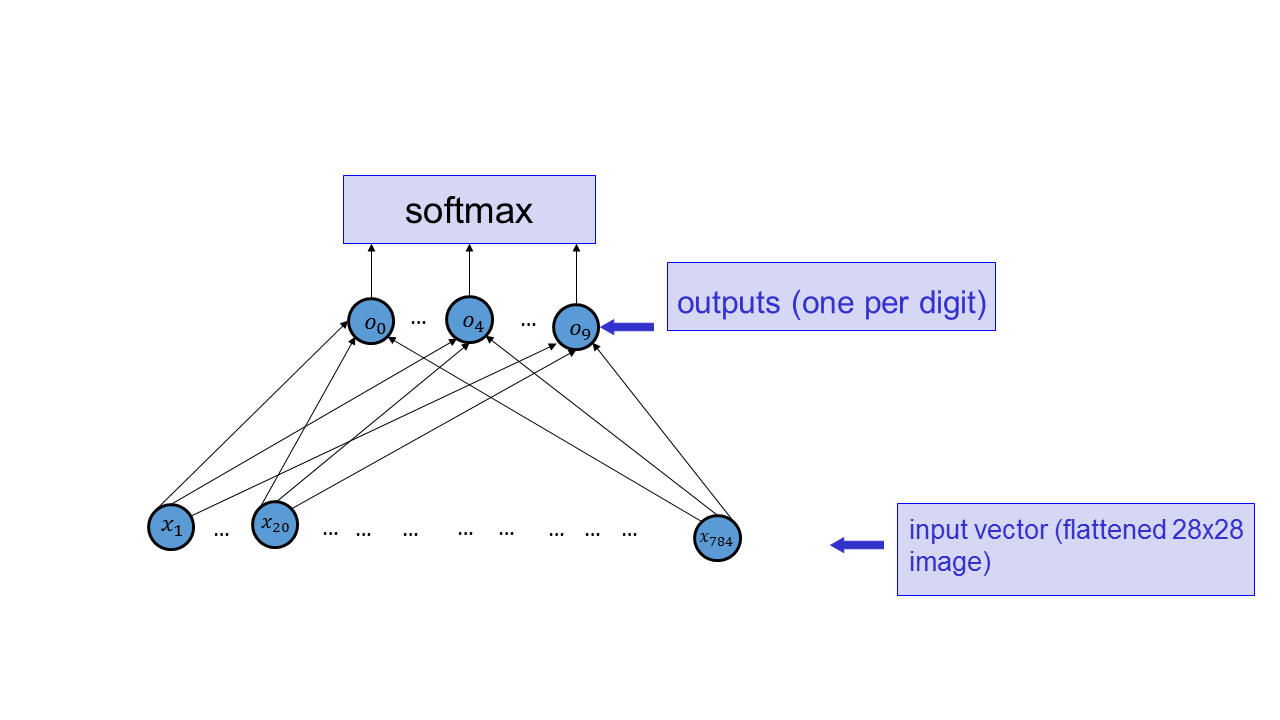
\includegraphics[scale=1, width=1\linewidth]{images/part2_simple_network}
	\caption{Simple network diagram from project handout.}
	\label{fig:part2_simple_network}
\end{figure}

\begin{figure}[!ht]
	\begin{lstlisting}
def softmax(y):
'''
Return the output of the softmax function for the matrix of output y. y
is an NxM matrix where N is the number of outputs for a single case, and M
is the number of cases
'''
return exp(y)/tile(sum(exp(y),0), (len(y),1))

def Part2(theta, X):
'''
Part2 returns the vectorized multiplication of the (n x 10) parameter matrix 
theta with the data X.

Arguments:
theta -- (n x 10) matrix of parameters (weights and biases)
x -- (n x 1) matrix whose rows correspond to pixels in images
'''

return softmax(np.dot(theta.T, X))
	\end{lstlisting}
	\caption{Python implementation of network using NumPy.}
	\label{fig:part2_code}
\end{figure}

\clearpage
\end{homeworkProblem}


% Part 3
\begin{homeworkProblem}
	\noindent \textit{Cost Function of Negative Log Probabilities}
	
	The Cost function that will be used for the network described in part 2 is:
	$$C = - \sum_{q = 1}^{m} (\sum_{l = 1}^{k} y_llog(p_l))_q$$
	Where $k$ is the number of output nodes, $m$ is the number of training samples, $p_l = \frac{e^{o_l}}{\sum_{c = 1}^{k} e^{o_c}}$ and $y_l$ is equal to $1$ if the training sample is labeled as $l$ and 0 otherwise.\newline
	\break
	
	\noindent \textit{Partial Derivative of the Cost Function (3a)}
	
	Let the matrix $W =  \begin{bmatrix}
    w_{11}       &w_{12} & w_{13} & \dots & w_{1k} \\
    w_{21}       &w_{22} & w_{23} & \dots & w_{2k} \\
    \hdotsfor{5} \\
    w_{n1}       &w_{n2} & w_{n3} & \dots & w_{nk}
\end{bmatrix}$ and let $W_j$ be the $j^{th}$ column of matrix $W$. This results in $o_j = W_j^Tx$ where
$x = \begin{bmatrix}
    x_{1} \\
    x_{2} \\
    \hdotsfor{1} \\
    x_{n} 
\end{bmatrix}$ and $n$ is equal to the number of pixels with an extra $1$ to multiply into the bias.\newline

	To calculate the partial derivative of C, we will consider only \textbf{a single training sample}: 
	$C = - \sum_{l = 1}^{k} y_llog(p_l)$
	The partial derivative with respect to $w_{ij}$ is:
	$$\frac{\partial C(W)}{\partial w_{ij}} = - \sum_{l = 1}^{k} \frac{\partial C}{\partial p_l}\frac{\partial p_l}{\partial o_j}\frac{\partial o_j}{\partial w_{ij}}$$
	The first term is straight forward: $\frac{\partial C}{\partial p_l} = \frac{y_l}{p_l}$.\newline
	
	For the second term, we have $\frac{\partial p_l}{\partial o_j} = 
	\begin{cases}\frac{-e^{o_l}e^{o_j}}{(\sum_{c = 1}^{k} e^{o_c})^2} = -p_lp_j, \text{if } l \ne j\\
	\frac{e^{o_j}}{\sum_{c = 1}^{k} e^{o_c}} - \frac{e^{2o_j}}{(\sum_{c = 1}^{k} e^{o_c})^2} = p_j - p_j^2, \text{if } l = j
	 \end{cases}$

	
	From the equation: $o_j = W_j^Tx$, we have $o_j = w_{1j}x_1 + w_{2j}x_2 + \dots + w_{nj}x_n$ and it is clear to see that: $\frac{\partial o_j}{\partial w_{ij}} = x_i$.\newline
	
	Putting it all together, we have:
	$$\frac{\partial C(W)}{\partial w_{ij}} = - (\sum_{l \ne j} (-\frac{y_l}{p_l}p_lp_j) + \frac{y_j}{p_j}(p_j - p_j^2))x_i = (\sum_{l \ne j} (y_lp_j) + y_j(p_j - 1))x_i$$
	Considering that we are using 1-hot encoding, only a single $y_l$ can equal 1. Therefore, $$\frac{\partial C(W)}{\partial w_{ij}} = \begin{cases}
    (p_j - 1)x_i,& \text{if } y_j = 1\\
    p_jx_i,              & \text{otherwise}
\end{cases}$$
Which is equivalent to saying: $\frac{\partial C(W)}{\partial w_{ij}} = (p_j - y_j)x_i$. To extend this to all training samples, we just have to sum up each individual contribution, resulting in the equation: $\frac{\partial C(W)}{\partial w_{ij}} = \sum_{q = 1}^{m}((p_j - y_j)x_i)_q$.
\clearpage

\noindent \textit{Vectorized Implementation of Gradient (3b)}

To vectorize the gradient, we first define the gradient matrix to be:  $$\frac{\partial C(W)}{\partial W} = 
\begin{bmatrix}
    \frac{\partial C}{w_{11}}       &\dots & \dots & \dots & \frac{\partial C}{w_{1k}} \\
    \frac{\partial C}{w_{21}}       &\dots & \dots & \dots & \frac{\partial C}{w_{2k}} \\
    \hdotsfor{5} \\
    \frac{\partial C}{w_{n1}}       &\dots & \dots & \dots & \frac{\partial C}{w_{nk}}
\end{bmatrix} = \begin{bmatrix}
    \sum_{q = 1}^{m}((p_1 - y_1)x_1)_q       &\dots & \dots & \dots & \sum_{q = 1}^{m}((p_k - y_k)x_1)_q \\
    \sum_{q = 1}^{m}((p_1 - y_1)x_2)_q       &\dots & \dots & \dots & \sum_{q = 1}^{m}((p_k - y_k)x_2)_q \\
    \hdotsfor{5} \\
    \sum_{q = 1}^{m}((p_1 - y_1)x_n)_q       &\dots & \dots & \dots & \sum_{q = 1}^{m}((p_k - y_k)x_n)_q
\end{bmatrix}$$

This is equivalent to: $ X(P - Y)^T$ where: $$X = \begin{bmatrix}
    x_{1}^{(1)}       & x_{1}^{(2)} & x_{1}^{(3)} & \dots & x_{1}^{(m)} \\
    x_{2}^{(1)}       & x_{2}^{(2)} & x_{2}^{(3)} & \dots & x_{2}^{(m)} \\
    \hdotsfor{5} \\
    x_{n}^{(1)}       & x_{n}^{(2)} & x_{n}^{(3)} & \dots & x_{n}^{(m)}
\end{bmatrix}
Y = \begin{bmatrix}
    y_{1}^{(1)}       & y_{1}^{(2)} & y_{1}^{(3)} & \dots & y_{1}^{(m)} \\
    y_{2}^{(1)}       & y_{2}^{(2)} & y_{2}^{(3)} & \dots & y_{2}^{(m)} \\
    \hdotsfor{5} \\
    y_{k}^{(1)}       & y_{k}^{(2)} & y_{k}^{(3)} & \dots & y_{k}^{(m)}
\end{bmatrix}
P =  \begin{bmatrix}
    p_{1}^{(1)}       & p_{1}^{(2)} & p_{1}^{(3)} & \dots & p_{1}^{(m)} \\
    p_{2}^{(1)}       & p_{2}^{(2)} & p_{2}^{(3)} & \dots & p_{2}^{(m)} \\
    \hdotsfor{5} \\
    p_{k}^{(1)}       & p_{k}^{(2)} & p_{k}^{(3)} & \dots & p_{k}^{(m)}
\end{bmatrix}$$
Where the superscript of each element represents the index of the training samples.
\clearpage
\end{homeworkProblem}


% Part 4
\begin{homeworkProblem}
	
\clearpage
\end{homeworkProblem}


% Part 5
\begin{homeworkProblem}
	
\clearpage
\end{homeworkProblem}


% Part 6
\begin{homeworkProblem}
	
\clearpage
\end{homeworkProblem}


% Part 7
\begin{homeworkProblem}
	
\clearpage
\end{homeworkProblem}


% Part 8
\begin{homeworkProblem}
	
\clearpage
\end{homeworkProblem}


% Part 9
\begin{homeworkProblem}
	
\clearpage
\end{homeworkProblem}


% Part 10
\begin{homeworkProblem}
	
\clearpage
\end{homeworkProblem}


%----------------------------------------------------------------------------------------

\end{document}